\section{Result and Analysis}
\begin{frame}{TIME EXECUTIONS}
	Total transmission time averages 49.91 ms.
	\vspace{-0.2cm}
	\begin{figure}
		\centering
		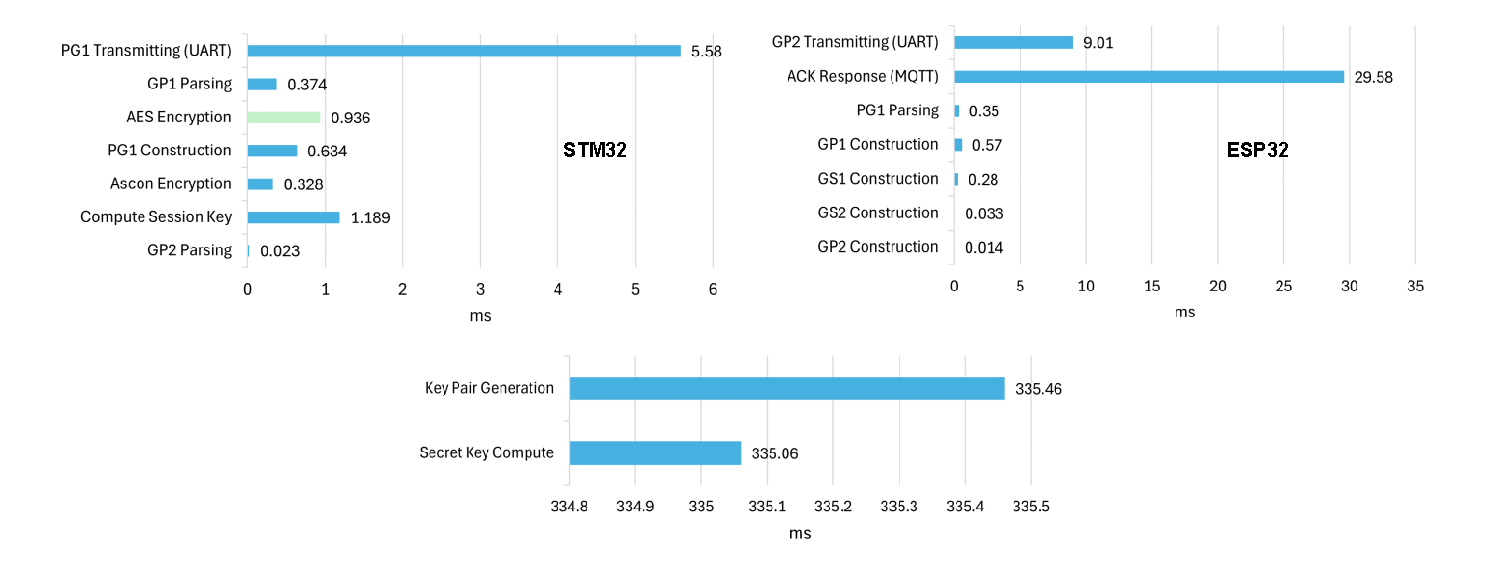
\includegraphics[width=1\textwidth]{pic/res_time.pdf}
	\end{figure}
\end{frame}

\begin{frame}{PACKET DELIVERY RATIO}
	\begin{figure}
		\centering
		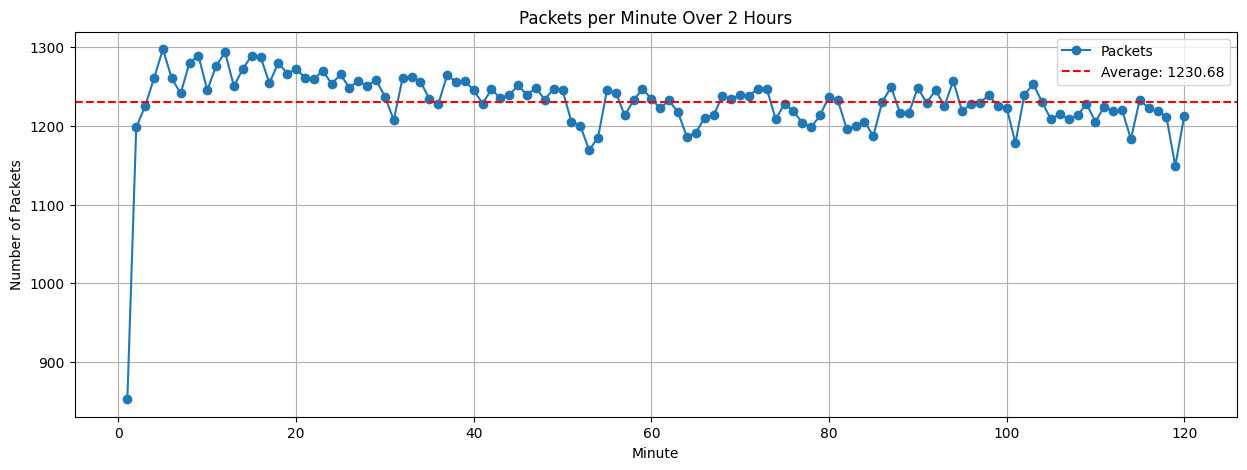
\includegraphics[width=0.65\textwidth]{pic/packet.png}
	\end{figure}
	\vspace{-0.3cm}
	\begin{figure}
		\centering
		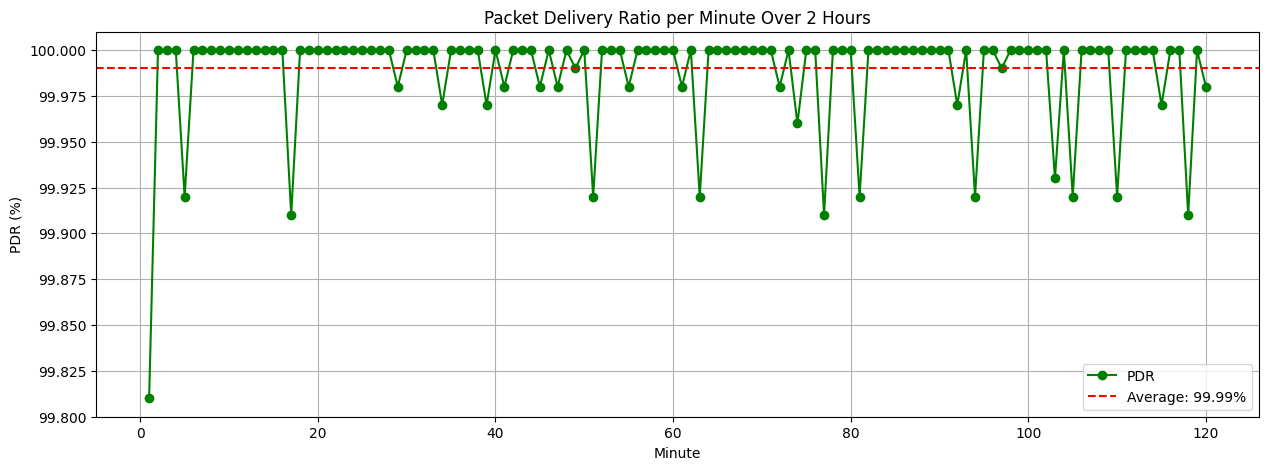
\includegraphics[width=0.65\textwidth]{pic/pdr.png}
	\end{figure}
\end{frame}

% \begin{frame}{POWER CONSUMPTION}
% 	\begin{figure}
% 		\centering
% 		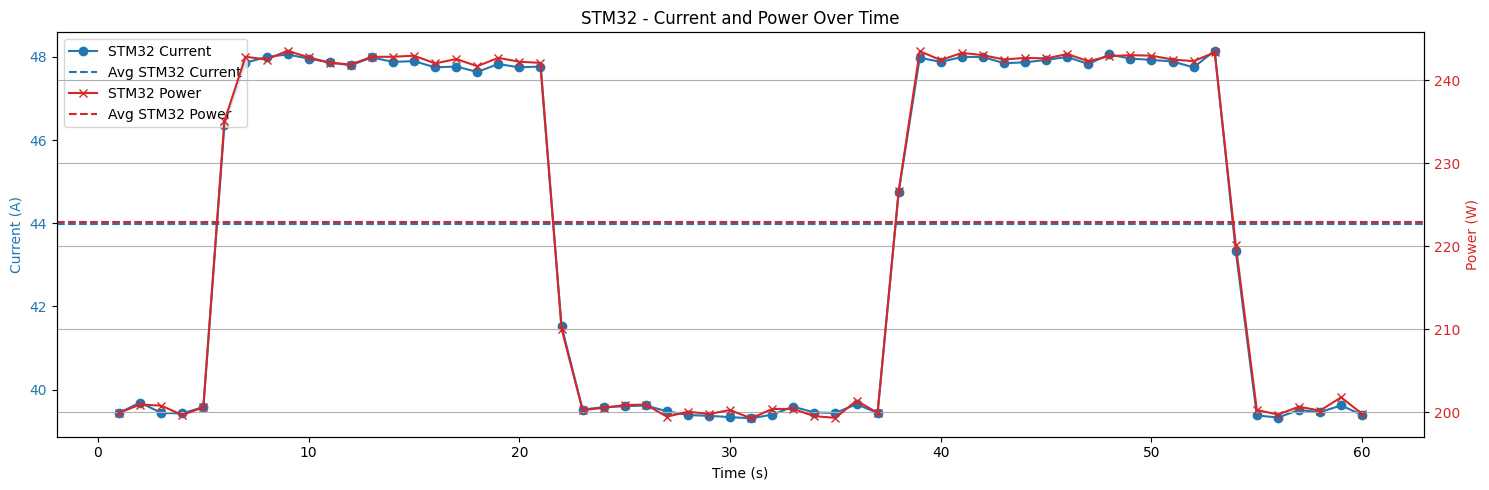
\includegraphics[width=0.7\textwidth]{pic/stm32power.png}
% 	\end{figure}
% 	\begin{figure}
% 		\centering
% 		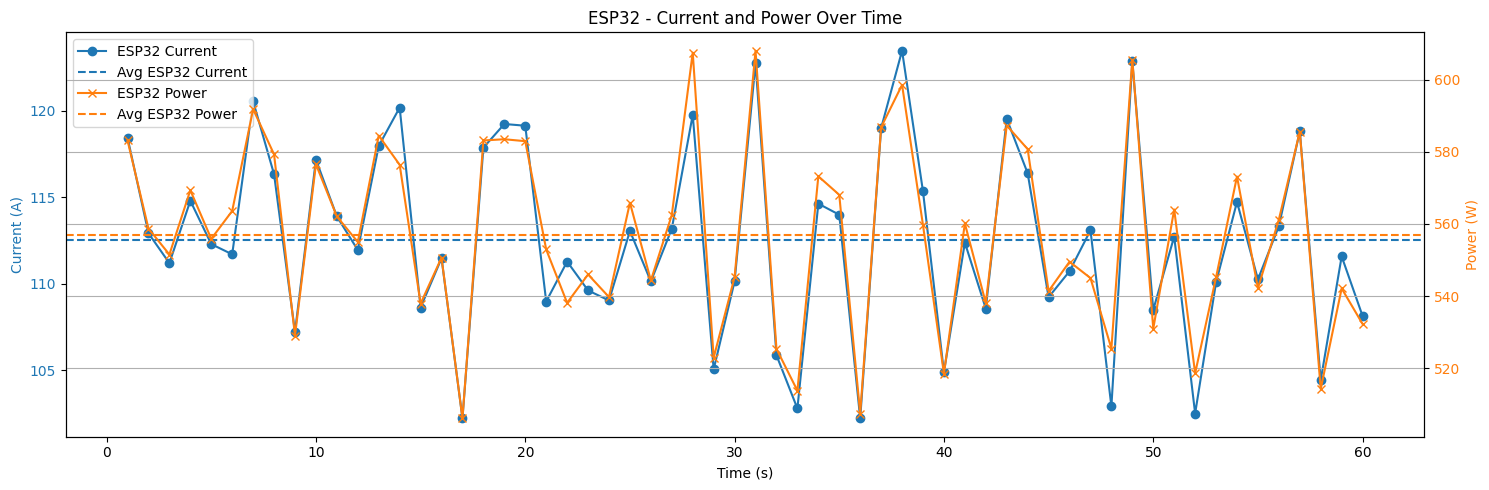
\includegraphics[width=0.7\textwidth]{pic/esp32power.png}
% 	\end{figure}
% \end{frame}

\begin{frame}{POWER CONSUMPTION}
	Total power consumption averages 779.43 mW.
	\vspace{-0.2cm}
	\begin{figure}
		\centering
		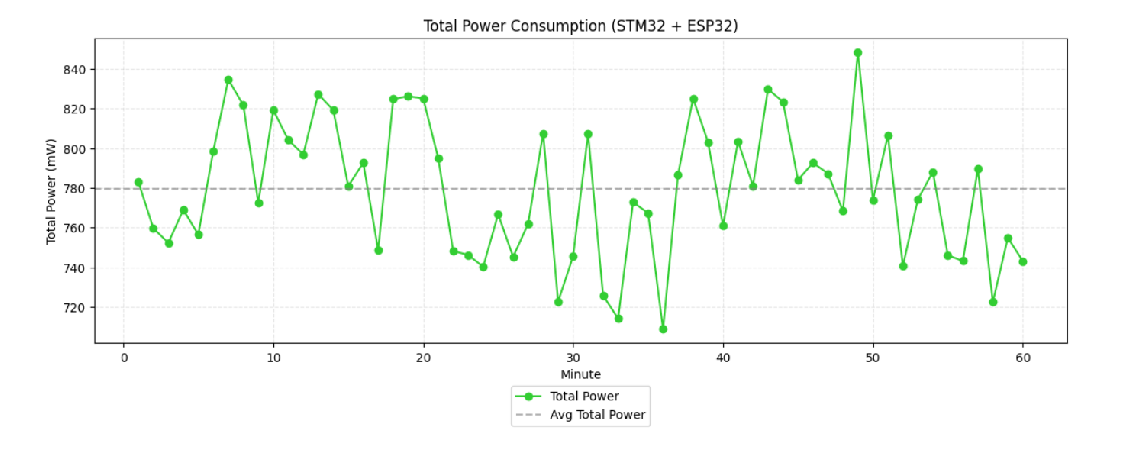
\includegraphics[width=0.85\textwidth]{pic/power.pdf}
	\end{figure}
\end{frame}

% \begin{frame}{PAYLOAD EFFICIENCY}
% 	Analyze based on the GS2 frame and 3 bytes data.
% 	\begin{figure}
% 		\centering
% 		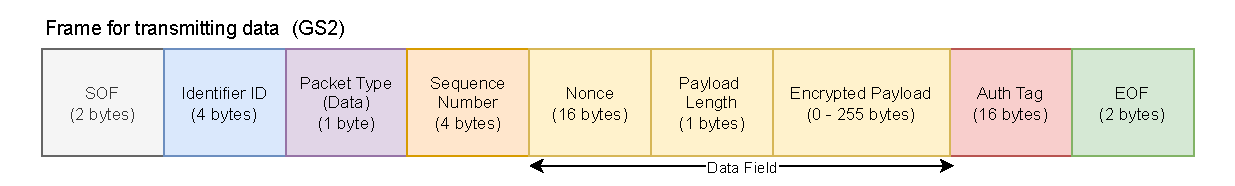
\includegraphics[width=1\textwidth]{pic/gs2.pdf}
% 	\end{figure}
% 	With 3 bytes data, total frame size is 49 bytes
% 	$\Rightarrow \text{Payload efficiency is } \frac{3}{49} \approx 6.12\%$
% \end{frame}

\begin{frame}{PAYLOAD EFFICIENCY}
	Analyze based on the GS2 frame.
	\begin{figure}
		\centering
		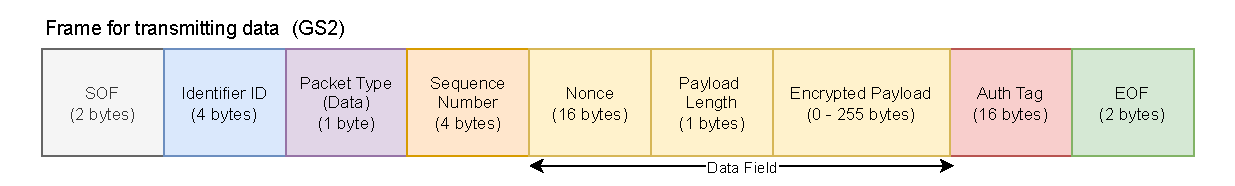
\includegraphics[width=1\textwidth]{pic/gs2.pdf}
	\end{figure}
	\vspace{-0.5cm}
	\begin{table}[h]
	\centering
	\small
	\caption{Payload efficiency with different payload lengths}
	\label{tab:efficiency}
	\begin{tabular}{|p{4cm}|p{5cm}|p{3cm}|}
	\hline
	Payload Length & Total Frame Size & Efficiency \\
	\hline
	3 bytes   & 49 bytes  & 6.12\%  \\
	10 bytes  & 56 bytes & 17.85\% \\
	20 bytes  & 66 bytes & 30.30\% \\
	50 bytes  & 96 bytes & 52.08\% \\
	\hline
	\end{tabular}
	\end{table}
	$\Rightarrow \text{The larger the payload, the higher the payload efficiency.}$
\end{frame}